\documentclass{beamer}

\usepackage{beamerthemesplit}
\usepackage{verbatim}

\usetheme{Pittsburgh}
%\usecolortheme{seagull}
%\usecolortheme{seahorse}
\usecolortheme{beaver}

\usefonttheme{serif}

\newcommand{\snT}{$(S/N)_{\textrm{size}}$}
%\newcommand{\snT}{$\left( \frac{S}{N}\right)_{\textrm{size}}$}
\newcommand{\snflux}{$(S/N)_{\textrm{flux}}$}
%\newcommand{\snflux}{$\left( \frac{S}{N}\right)_{\textrm{flux}}$}

\newcommand{\vecg}{\mbox{\boldmath $g$}}
\newcommand{\vecQ}{\mbox{\boldmath $Q$}}
\newcommand{\matR}{\mbox{$\bf R$}}
\newcommand{\matC}{\mbox{$\bf C$}}
\newcommand{\sersic}{S\'{e}rsic}
\newcommand{\devauc}{De Vaucouleurs'}

\newcommand{\probwts}{\texttt{ProbWTS}}


\title{Stacked Weak Lensing with Redmapper Clusters in Early DES Data}
\author{Erin Sheldon}
\institute{Brookhaven National Laboratory}

% http://texblog.net/latex-archive/plaintex/beamer-footline-frame-number/
% to add the page (frame ) number and not screw up the bottom line
% works for split themes?
%\expandafter\def\expandafter\insertshorttitle\expandafter{%
%      \insertshorttitle\hfill%
%        \insertframenumber\,/\,\inserttotalframenumber}


\begin{document}

\frame{\titlepage}

\frame{
    \frametitle{Outline}

    \fontsize{12}{1.5\baselineskip}

    \begin{itemize}

        \item Motivation to stack clusters
        \item Results drawn from the wiki:
        \item {\small https://cdcvs.fnal.gov/redmine/projects/des-clusters/wiki/
            WL\_with\_RedMapper\_in\_Early\_DES\_Data}
        \item JBOP (Just a Bunch of Plots)
        \item TODO

    \end{itemize}
}

\frame{
    \frametitle{Motivation for Stacking}
    \begin{itemize}

        \item Simplify interpretation: all projections and neighboring structure are
            part of the well-understood 2-halo term

        \item ``Universal Profile'' from theory/sims is really a description of the mean
            profile, which stacking measures.

        \item Corrections are possible:
            \begin{itemize}

                \item ``boost factors'': sources clustered with the lenses give
                    zero shear; this can be corrected using the
                    cross-correlation function. (e.g. Sheldon 2009)

                \item Some additive errors show up in random point tests, and can
                    be subtracted. (e.g. Sheldon 2009)

                \item mis-centering can be understood statistically and corrected
                    in the ensemble average (Rozo in prep.) or modeled (Johnston 2007)

                \item non-sphericity averaged out and remaining orientation
                    bias can be modeled (Dietrich 2014)

            \end{itemize}

    \end{itemize}
}
\frame{
    \frametitle{Stacked Signal for RedMapper Clusters}
    \includegraphics[width=\textwidth]{binned-rmdes01im3shape-r01-lambda-12-allplot.pdf}
    \newline
    Erin Sheldon
}

\frame{
    \frametitle{Stacked Signal for RedMapper Clusters: B mode}
    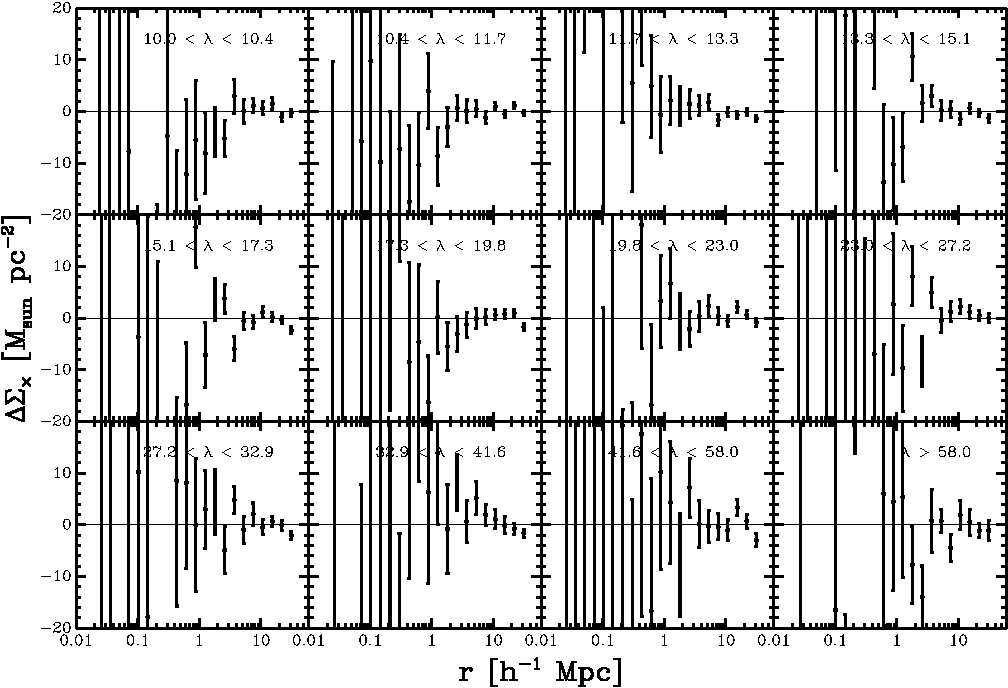
\includegraphics[width=\textwidth]{binned-rmdes01im3shape-r01-lambda-12-osig-allplot.pdf}
    \newline
    Erin Sheldon
}



\frame{
    \frametitle{Stacked Signal for RedMapper Clusters}
    \begin{columns}
        \begin{column}{0.4\textwidth}
            \begin{itemize}
                \item Im3Shape catalog v4 with suggested cuts
                \item No boost corrections yet applied
                \item Mis-centering not accounted for.
                \item Potential photometry problems in crowded fields.
            \end{itemize}
        \end{column}

        \begin{column}{0.6\textwidth}
            \includegraphics[width=\textwidth]{binned-rmdes01im3shape-r01-lambda-12-allplot.pdf}
        \newline
        Erin Sheldon
        \end{column}
    \end{columns}
}


\frame{
    \frametitle{Dominik's Shape Consistency Tests}
    \begin{columns}
        \begin{column}{0.4\textwidth}
            \begin{itemize}
                \item Larger galaxies have larger detected shear.
                \item Partly related to definition of size
            \end{itemize}
        \end{column}

        \begin{column}{0.6\textwidth}
            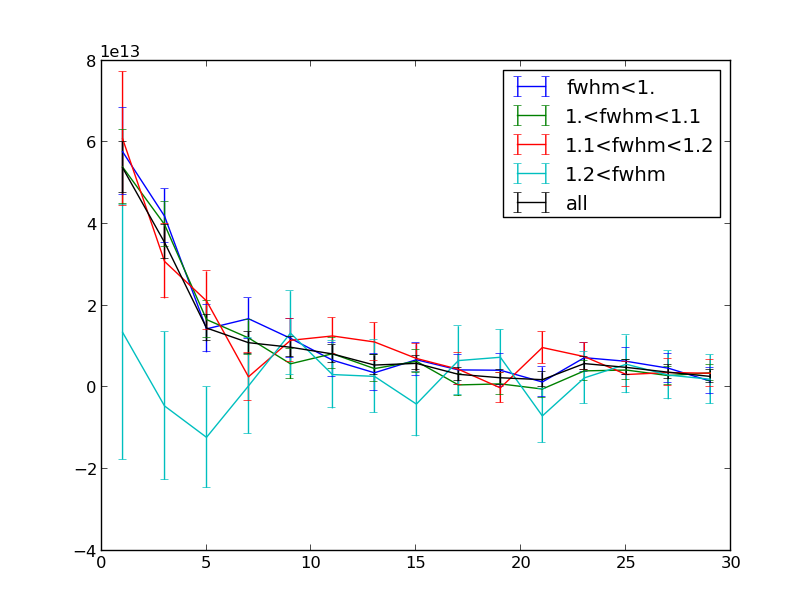
\includegraphics[width=\textwidth]{i_fwr.png}
        \newline
        Dominik Gangkofner
        \end{column}
    \end{columns}
}

\frame{
    \frametitle{Peter's Consistency Tests}
    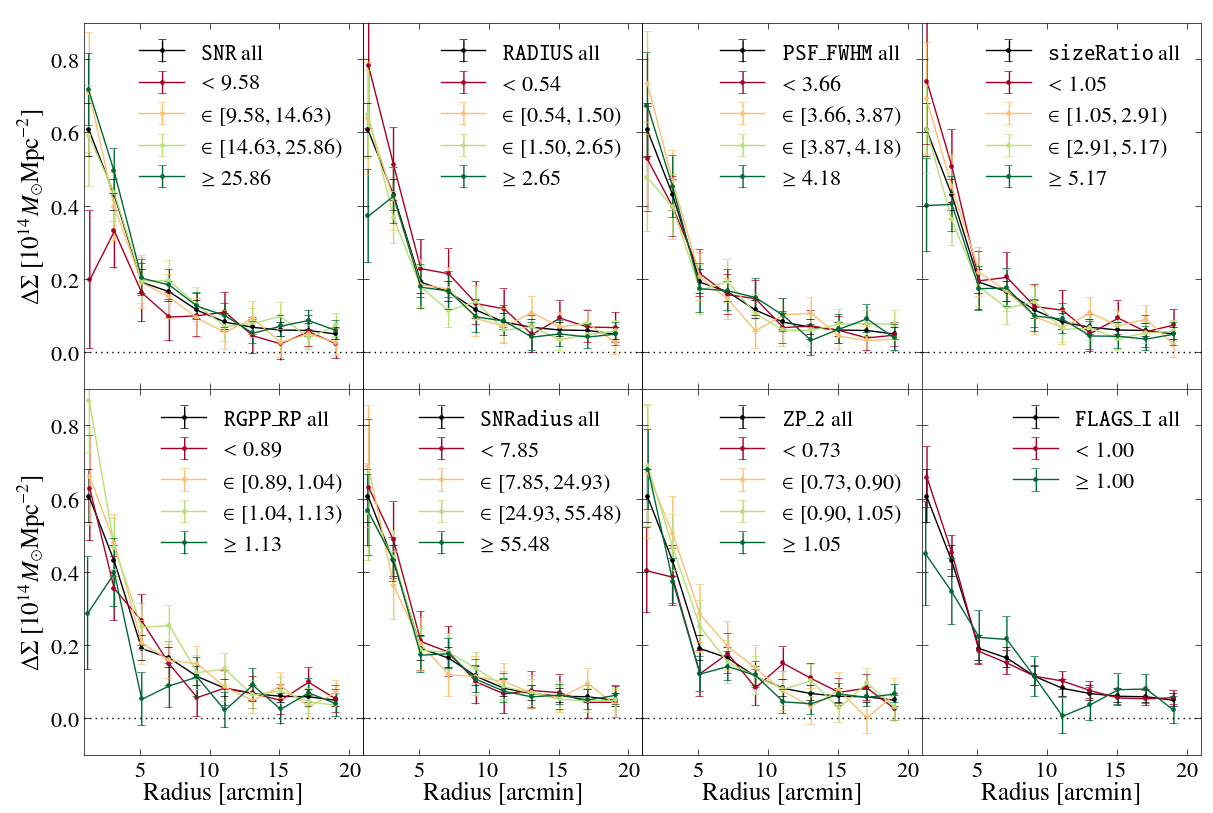
\includegraphics[width=\textwidth]{redmapper_lgt20_z0_1_0_8_im3shape_i_gold.png}
    \newline
    Peter Melchior
}


\frame{
    \frametitle{Peter's Consistency Tests}

    \begin{itemize}
        \item There is a clear dependence on SNR.  No noise bias correction applied.

        \item Galaxies with smaller RADIUS (deconvolved half-light radius) are
            more strongly lensed, in particular at larger separation from the
            cluster centers.

        \item 

            Blending (FLAGS=1) does matter a lot towards cluster centers. This
            was also seen in the pointed SV clusters.
            This FLAG==0 cut needs to be applied for any lens sample that is
            associated with a higher concentration of galaxies.
        \item flag==0 cut
            does introduce a density-dependent bias: see this paper

    \end{itemize}
}

\frame{
    \frametitle{Jeorg's Coadd Tile Consistency Tests}

    \begin{itemize}
        \item Check that the shear catalog properties of different DES tiles are consistent. 
        \item Computing the KS test for several galaxy properties. 
    \end{itemize}

}

\frame{
    \frametitle{Jeorg's Coadd Tile Consistency Tests}
    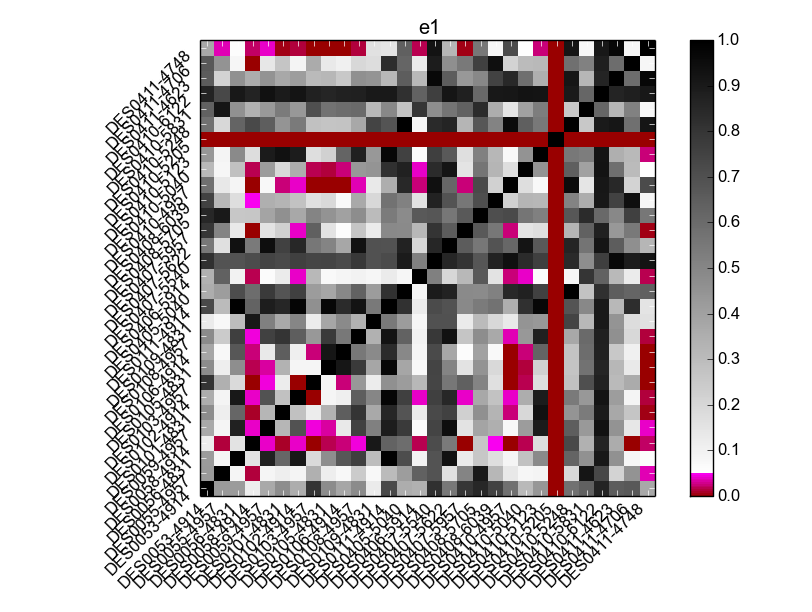
\includegraphics[width=\textwidth]{e1_KS.png}
    \newline
    Jeorg Deitrich
}

\frame{
    \frametitle{Jeorg's Coadd Tile Consistency Tests}
    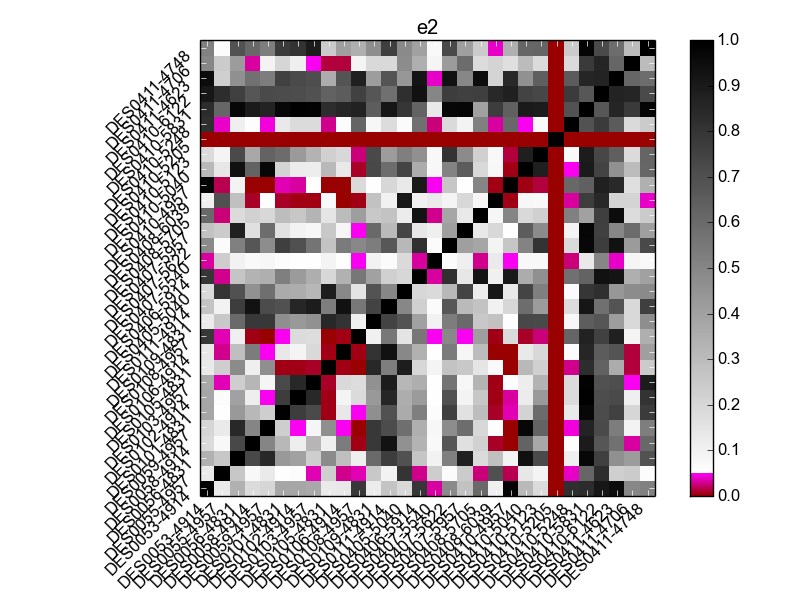
\includegraphics[width=\textwidth]{e2_KS.png}
    \newline
    Jeorg Deitrich
}

\frame{
    \frametitle{Jeorg's Coadd Tile Consistency Tests}
    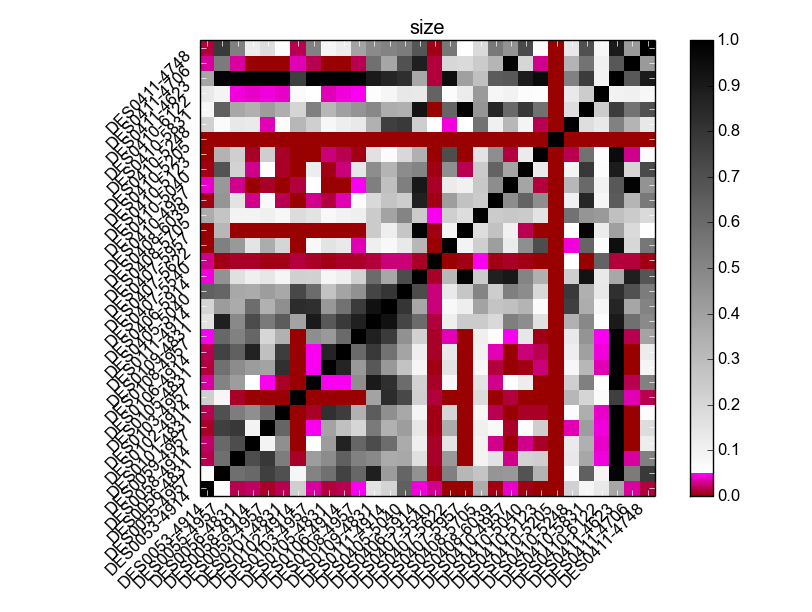
\includegraphics[width=\textwidth]{size_KS.png}
    \newline
    Jeorg Deitrich
}

\frame{
    \frametitle{TODO}

    \fontsize{12}{1.5\baselineskip}

    \begin{itemize}

        \item Run on new RedMapper catalogs.
        \item Run with new im3shape v5 (collating), ngmix (running)
        \item Repeat above tests.
        \item Add random points tests:  Randoms are special for RedMapper

    \end{itemize}
}



\end{document}
